% UML 图集 — 基于大模型的智能文件管理与智能体协同平台
% 编译: xelatex uml.tex && xelatex uml.tex
\documentclass[a4paper,zihao=-4]{ctexart}
\usepackage[top=1.5cm,bottom=1.5cm,left=1.5cm,right=1.5cm]{geometry}
\usepackage{tikz}
\usepackage{booktabs}
\usepackage{hyperref}
\usetikzlibrary{
  arrows.meta, positioning, shapes.geometric, shapes.multipart,
  calc, fit, backgrounds, decorations.pathreplacing, shadows,
  chains, matrix
}

\hypersetup{colorlinks=true,linkcolor=blue}

\begin{document}

% ============================================================
% 图 1：系统整体架构组件图
% ============================================================
\section*{图1：系统整体架构组件图}

\vspace{1em}
\begin{center}
\begin{tikzpicture}[
  node distance=8mm and 10mm,
  comp/.style={rectangle, draw, rounded corners=4pt, fill=blue!8,
               minimum width=28mm, minimum height=10mm, align=center,
               font=\small\sffamily},
  infra/.style={rectangle, draw, rounded corners=4pt, fill=green!10,
                minimum width=30mm, minimum height=9mm, align=center,
                font=\small\sffamily},
  store/.style={cylinder, shape border rotate=90, draw, fill=yellow!10,
                minimum width=28mm, minimum height=12mm, align=center,
                font=\small\sffamily},
  arrow/.style={-{Stealth}, thick, gray},
]

% ---- 前端层 ----
\node[comp, fill=orange!12, minimum width=126mm, minimum height=8mm,
      font=\small\bfseries\sffamily] (frontend) at (0,6)
      {Web 前端 (Vue 3 + Naive UI + Vue Flow)};

\node[comp, fill=orange!20] (fe-file) at (-5,4.5)  {文件管理界面};
\node[comp, fill=orange!20] (fe-qa)   at (2,4.5)   {知识问答对话窗};
\node[comp, fill=orange!20] (fe-flow) at (-5,3)    {工具流编排器};
\node[comp, fill=orange!20] (fe-team) at (2,3)     {团队空间·聊天};
\node[comp, fill=orange!20] (fe-agent) at (-1.5,1.5) {智能体执行面板};

% ---- 后端层 ----
\node[comp, fill=blue!12, minimum width=126mm, minimum height=8mm,
      font=\small\bfseries\sffamily] (backend) at (0,-1.5)
      {后端服务 (Python FastAPI)};

\node[comp, fill=blue!20] (be-file) at (-5,-3)    {文件管理服务};
\node[comp, fill=blue!20] (be-rag)  at (2,-3)     {RAG 引擎};
\node[comp, fill=blue!20] (be-agent) at (-5,-4.5) {智能体编排器};
\node[comp, fill=blue!20] (be-flow) at (2,-4.5)   {工具流引擎};
\node[comp, fill=blue!20] (be-team) at (-1.5,-6)  {团队协作服务};

% ---- 基础设施层 ----
\node[infra, fill=green!12, minimum width=126mm, minimum height=8mm,
      font=\small\bfseries\sffamily] (infra) at (0,-8)
      {共享基础设施};

\node[infra, fill=green!20] (i-llm)  at (-5,-9.5)  {LLM 调用网关};
\node[infra, fill=green!20] (i-vec)  at (2,-9.5)   {向量数据库\\FAISS / Milvus};
\node[infra, fill=green!20] (i-ws)   at (-1.5,-11) {WebSocket 消息推送};

% ---- 存储层 ----
\node[store] (db)    at (-3.5,-13.5) {MySQL 8.0\\元数据·权限·消息};
\node[store] (minio) at (3.5,-13.5)  {MinIO / 本地\\文件实体存储};

% ---- 层间连线 ----
\draw[arrow] (fe-file.south)  -- (be-file.north);
\draw[arrow] (fe-qa.south)    -- (be-rag.north);
\draw[arrow] (fe-agent.south) -- (be-agent.north);
\draw[arrow] (fe-flow.south)  -- (be-flow.north);
\draw[arrow] (fe-team.south)  -- (be-team.north);
\draw[arrow] (be-rag.south)   -- (i-llm.north);
\draw[arrow] (be-rag.south)   -- (i-vec.north);
\draw[arrow] (be-agent.south) -- (i-llm.north);
\draw[arrow] (be-flow.south)  -- (i-ws.north);
\draw[arrow] (be-team.south)  -- (i-ws.north);
\draw[arrow] (be-file.south)  -- (minio.north);
\draw[arrow] (i-vec.south)    -- (db.north);
\draw[arrow] (i-ws.south)     -- (db.north);

% ---- 协议标注 ----
\node[font=\footnotesize\ttfamily, text=gray] at (6.5, 6)
     {REST / WebSocket};

\end{tikzpicture}
\end{center}

\newpage

% ============================================================
% 图 2：用例图
% ============================================================
\section*{图2：系统用例图}

\vspace{1em}
\begin{center}
\begin{tikzpicture}[
  actor/.style={rectangle, draw, rounded corners=3pt, fill=gray!12,
                minimum width=18mm, minimum height=8mm, align=center,
                font=\small},
  usecase/.style={ellipse, draw, fill=blue!8, minimum width=26mm,
                  minimum height=10mm, align=center, font=\small\sffamily},
  sys/.style={rectangle, draw=gray, dashed, inner sep=10mm,
              rounded corners=8pt, minimum width=100mm, minimum height=58mm},
  arrow/.style={-{Stealth}, thick},
  inh/.style={thick, dashed, -{Stealth}},
]

% ---- 系统边界 ----
\node[sys, label=above:{\textbf{系统边界}}] (boundary) at (0,0) {};

% ---- 角色 ----
\node[actor] (admin) at (-6.5,  3)   {管理员};
\node[actor] (user)  at (-6.5,  0)   {普通用户};
\node[actor] (team)  at (-6.5, -3)   {团队成员};

% ---- 用例 ----
\node[usecase] (uc-upload) at (0,  5)    {文件上传管理};
\node[usecase] (uc-search) at (4,  5)    {全文搜索};
\node[usecase] (uc-qa)     at (0,  2.5)  {知识库问答};
\node[usecase] (uc-agent)  at (4,  2.5)  {智能体任务编排};
\node[usecase] (uc-flow)   at (0,  0)    {工具流编排};
\node[usecase] (uc-team)   at (4,  0)    {团队协作};
\node[usecase] (uc-perm)   at (0, -2.5)  {权限管理};
\node[usecase] (uc-tool)   at (4, -2.5)  {工具注册管理};
\node[usecase] (uc-chat)   at (2, -4.5)  {实时聊天};

% ---- 连线 ----
\draw[arrow] (admin) -- (uc-perm);
\draw[arrow] (admin) -- (uc-tool);
\draw[arrow] (user)  -- (uc-upload);
\draw[arrow] (user)  -- (uc-search);
\draw[arrow] (user)  -- (uc-qa);
\draw[arrow] (user)  -- (uc-agent);
\draw[arrow] (user)  -- (uc-flow);
\draw[arrow] (team)  -- (uc-team);
\draw[arrow] (team)  -- (uc-chat);
\draw[arrow] (team)  -- (uc-upload);

% ---- 继承 ----
\draw[inh] (team) -- (user) node[midway, left, font=\footnotesize] {<<继承>>};

\end{tikzpicture}
\end{center}

\newpage

% ============================================================
% 图 3：数据库 ER 图
% ============================================================
\section*{图3：数据库核心 ER 图}

\vspace{1em}
\begin{center}
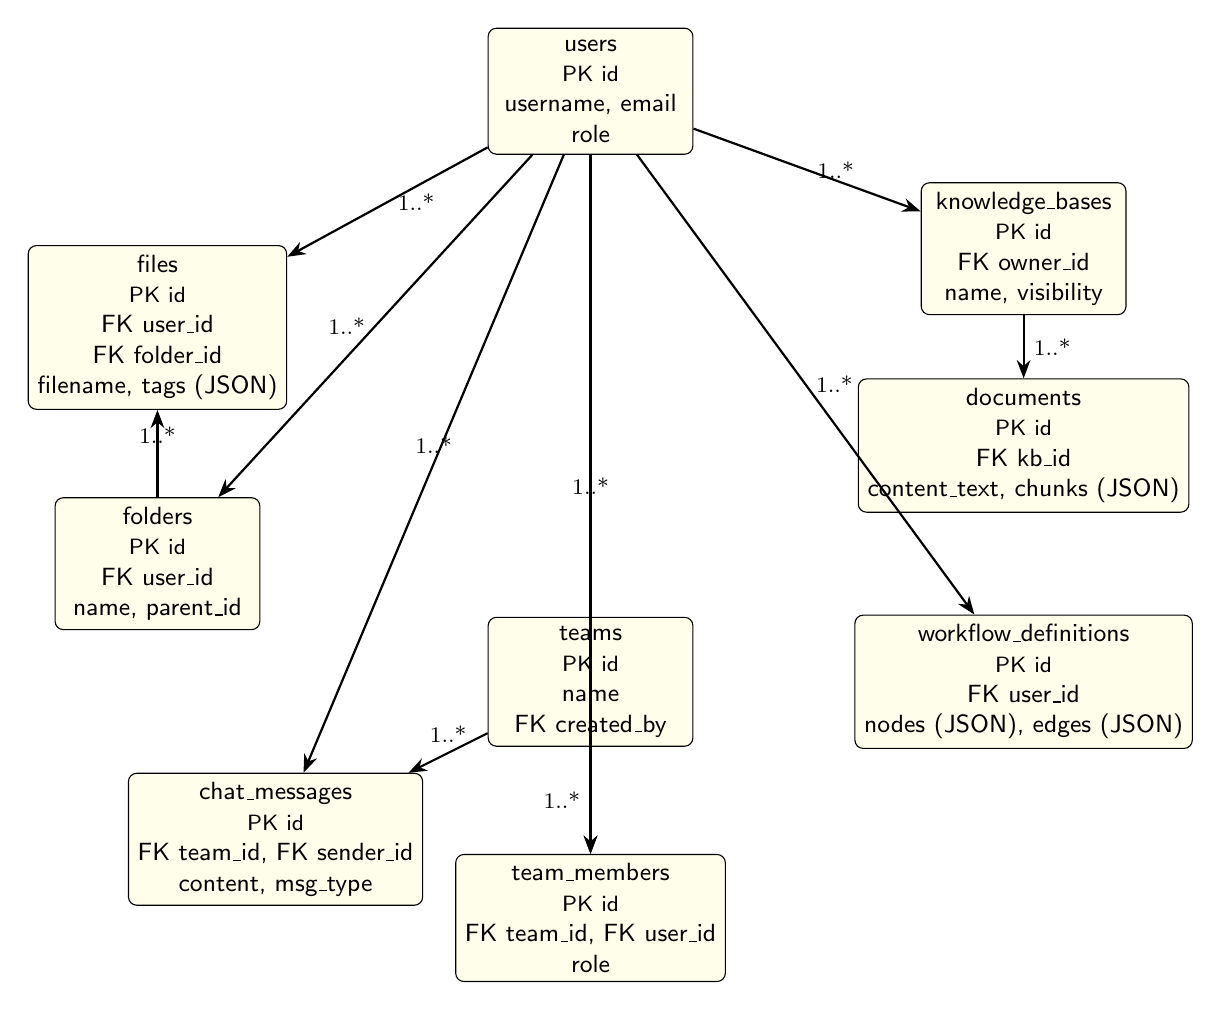
\begin{tikzpicture}[
  entity/.style={rectangle, draw, rounded corners=3pt, fill=yellow!8,
                 minimum width=26mm, minimum height=16mm, align=center,
                 font=\small\sffamily},
  rel/.style={thick, -{Stealth}},
]

% ---- 实体 ----
\node[entity] (users)  at (0,6)     {users\\ \footnotesize PK id\\username, email\\role};

\node[entity] (files)  at (-5.5,3)  {files\\ \footnotesize PK id\\FK user\_id\\FK folder\_id\\filename, tags (JSON)};

\node[entity] (folders) at (-5.5,0) {folders\\ \footnotesize PK id\\FK user\_id\\name, parent\_id};

\node[entity] (teams)   at (0,-1.5) {teams\\ \footnotesize PK id\\name\\FK created\_by};

\node[entity] (tm)      at (0,-4.5) {team\_members\\ \footnotesize PK id\\FK team\_id, FK user\_id\\role};

\node[entity] (kb)      at (5.5,4)  {knowledge\_bases\\ \footnotesize PK id\\FK owner\_id\\name, visibility};

\node[entity] (docs)    at (5.5,1.5){documents\\ \footnotesize PK id\\FK kb\_id\\content\_text, chunks (JSON)};

\node[entity] (wf)      at (5.5,-1.5){workflow\_definitions\\ \footnotesize PK id\\FK user\_id\\nodes (JSON), edges (JSON)};

\node[entity] (chat)    at (-4,-3.5){chat\_messages\\ \footnotesize PK id\\FK team\_id, FK sender\_id\\content, msg\_type};

% ---- 关系 ----
\draw[rel] (users)  -- (files)   node[midway, right, font=\footnotesize] {1..*};
\draw[rel] (users)  -- (folders) node[midway, left,  font=\footnotesize] {1..*};
\draw[rel] (users)  -- (kb)      node[midway, right, font=\footnotesize] {1..*};
\draw[rel] (users)  -- (chat)    node[midway, above, font=\footnotesize] {1..*};
\draw[rel] (folders)-- (files)   node[midway, above, font=\footnotesize] {1..*};
\draw[rel] (kb)     -- (docs)    node[midway, right, font=\footnotesize] {1..*};
\draw[rel] (teams)  -- (tm)      node[midway, left,  font=\footnotesize] {1..*};
\draw[rel] (users)  -- (tm)      node[midway, above, font=\footnotesize] {1..*};
\draw[rel] (teams)  -- (chat)    node[midway, above, font=\footnotesize] {1..*};
\draw[rel] (users)  -- (wf)      node[midway, right, font=\footnotesize] {1..*};

\end{tikzpicture}
\end{center}

\newpage

% ============================================================
% 图 4：智能体 ReAct 序列图
% ============================================================
\section*{图4：智能体 ReAct 任务编排序列图}

\vspace{1em}
\begin{center}
\begin{tikzpicture}[
  actor/.style={rectangle, draw, fill=gray!12, minimum width=18mm,
                minimum height=7mm, align=center, font=\small\sffamily},
  lifeline/.style={draw=gray, dotted, thick},
  msg/.style={-{Stealth}, thick},
]

% ---- 参与对象 ----
\node[actor] (user)  at (0,0)     {用户};
\node[actor] (agent) at (4.5,0)   {Agent 编排器};
\node[actor] (llm)   at (9,0)     {LLM};
\node[actor] (tools) at (13.5,0)  {工具集};

% ---- 生命线 ----
\foreach \x in {0,4.5,9,13.5}
  \draw[lifeline] (\x,-0.5) -- (\x,-17.5);

% ---- 消息序列 ----
% 输入
\draw[msg] (0,-1.0)  -- node[above, font=\small] {① 自然语言输入} (4.5,-1.0);
\draw[msg] (4.5,-1.8)-- node[above, font=\small] {② Prompt + 工具列表} (9,-1.8);

% Thought
\draw[msg] (9,-3.0)  -- node[above, font=\small] {③ Thought: 需要查文件} (4.5,-3.0);

% Action → Tool
\draw[msg] (4.5,-4.2)-- node[above, font=\small] {④ Action: file\_search(keyword)} (13.5,-4.2);

% Observation
\draw[msg] (13.5,-5.8) -- node[above, font=\small] {⑤ Observation: [file1, file2]} (4.5,-5.8);

% Send to LLM again
\draw[msg] (4.5,-7.0) -- node[above, font=\small] {⑥ Prompt + 检索结果} (9,-7.0);

% Second round
\draw[msg] (9,-8.5)  -- node[above, font=\small] {⑦ Thought: 需要知识问答} (4.5,-8.5);
\draw[msg] (4.5,-9.8)-- node[above, font=\small] {⑧ Action: knowledge\_qa(files)} (13.5,-9.8);
\draw[msg] (13.5,-11.4) -- node[above, font=\small] {⑨ Observation: 答案文本} (4.5,-11.4);

% Final answer
\draw[msg] (4.5,-12.5) -- node[above, font=\small] {⑩ Prompt + 汇总} (9,-12.5);
\draw[msg] (9,-14.0)   -- node[above, font=\small] {⑪ Answer: 最终回答} (4.5,-14.0);
\draw[msg] (4.5,-15.0) -- node[above, font=\small] {⑫ 呈现最终答案} (0,-15.0);

% ---- 循环标注 ----
\draw[decorate, decoration={brace, amplitude=6pt, mirror}, thick]
  (15,-3.5) -- (15,-12) node[midway, right=10pt, font=\small, align=left]
  {ReAct 循环\\Thought → Action\\→ Observation\\可多次迭代};

\end{tikzpicture}
\end{center}

\newpage

% ============================================================
% 图 5：工具流 DAG 示例
% ============================================================
\section*{图5：工具流 DAG 示例 —— 新文件自动摘要流程}

\vspace{1em}
\begin{center}
\begin{tikzpicture}[
  node distance=10mm and 18mm,
  tnode/.style={rectangle, draw, rounded corners=4pt, fill=blue!10,
                minimum width=32mm, minimum height=11mm, align=center,
                font=\small\sffamily},
  cnode/.style={diamond, draw, fill=orange!12, minimum width=22mm,
                minimum height=14mm, align=center, font=\small\sffamily},
  onode/.style={rectangle, draw, rounded corners=4pt, fill=green!10,
                minimum width=32mm, minimum height=10mm, align=center,
                font=\small\sffamily},
  arrow/.style={-{Stealth}, thick},
]

% ---- 节点 ----
\node[onode] (start) {开始\\\footnotesize (事件触发：新文件上传)};

\node[tnode, below=of start] (parse) {文件解析\\\footnotesize 提取文本 + 元数据};

\node[tnode, below=of parse] (ocr) {OCR 识别\\\footnotesize PaddleOCR 提取图中文字};

\node[cnode, below=of ocr] (check) {文件类型?};

\node[tnode, below left=of check, xshift=-8mm] (embed) {向量化入库\\\footnotesize BGE-M3 → FAISS};

\node[tnode, below right=of check, xshift=8mm] (tag) {自动打标签\\\footnotesize 基于内容分类};

\node[tnode, below=of embed] (summary) {LLM 摘要生成\\\footnotesize 生成文件摘要};

\node[onode, below=of summary] (notify) {通知用户\\\footnotesize WebSocket 推送\\摘要 + 标签};

% ---- 连线 ----
\draw[arrow] (start)  -- (parse);
\draw[arrow] (parse)  -- (ocr);
\draw[arrow] (ocr)    -- (check);
\draw[arrow] (check)  -- node[above left, font=\small] {文档类} (embed);
\draw[arrow] (check)  -- node[above right, font=\small] {图片类} (tag);
\draw[arrow] (embed)  -- (summary);
\draw[arrow] (tag)    |- (summary);
\draw[arrow] (summary)-- (notify);

% ---- 并行标注 ----
\draw[decorate, decoration={brace, amplitude=6pt}, thick, gray]
  ($(embed.west)+(-6mm,0)$) -- ($(tag.east)+(6mm,0)$)
  node[midway, above=6pt, font=\small] {并行执行};

\end{tikzpicture}
\end{center}

\newpage

% ============================================================
% 图 6：权限 RBAC 模型
% ============================================================
\section*{图6：RBAC 权限模型}

\vspace{1em}
\begin{center}
\begin{tikzpicture}[
  box/.style={rectangle, draw, rounded corners=3pt, fill=blue!8,
              minimum width=22mm, minimum height=10mm, align=center,
              font=\small\sffamily},
  arrow/.style={-{Stealth}, thick},
]

\node[box, fill=orange!12] (user) {用户 (User)};

\node[box, below left=16mm and 8mm of user]  (role) {角色 (Role)};
\node[box, below right=16mm and 8mm of user] (perm) {权限 (Permission)};

\node[box, below=16mm of role]   (resource) {资源 (Resource)\\文件/文件夹/知识库/工具};
\node[box, below=16mm of perm]   (action)   {操作 (Action)\\read/write/delete/manage};

\node[box, below=28mm of user, fill=green!10, minimum width=65mm]
  (acl) {ACL 权限检查中间件\\Token → 角色 → 资源权限 → 放行/拒绝};

% ---- 关系 ----
\draw[arrow] (user) -- node[left, font=\small] {N:M} (role);
\draw[arrow] (role) -- node[right, font=\small] {N:M} (perm);
\draw[arrow] (perm) -- (resource);
\draw[arrow] (perm) -- (action);
\draw[arrow, bend right=20] (user.south) to node[midway, right, font=\small]
  {直接授权(可选)} (perm.east);

% ---- 包围框 ----
\draw[decorate, decoration={brace, amplitude=6pt}, thick]
  ($(role.west)+(-5mm,8mm)$) -- ($(perm.east)+(5mm,8mm)$)
  node[midway, above=6pt, font=\small\bfseries] {RBAC 核心};

\end{tikzpicture}
\end{center}

\newpage

% ============================================================
% 图 7：团队协作状态图
% ============================================================
\section*{图7：团队协作活动流程}

\vspace{1em}
\begin{center}
\begin{tikzpicture}[
  state/.style={rectangle, draw, rounded corners=6pt, fill=blue!8,
                minimum width=30mm, minimum height=10mm, align=center,
                font=\small\sffamily},
  arrow/.style={-{Stealth}, thick},
]

\node[state, fill=green!10] (create)  {创建团队\\\footnotesize 管理员发起};

\node[state, below=12mm of create] (invite)  {邀请成员\\\footnotesize 链接/邮箱邀请};

\node[state, below=12mm of invite] (join)    {成员加入\\\footnotesize 分配角色};

\node[state, below=12mm of join] (folder)   {创建团队文件夹\\\footnotesize 设置权限};

\node[state, right=30mm of folder, fill=orange!12] (upload)  {文件上传\\\footnotesize 自动可见};

\node[state, above=12mm of upload, fill=orange!12] (annotate){协作批注\\\footnotesize 讨论反馈};

\node[state, above=12mm of annotate, fill=orange!12] (chat)   {实时聊天\\\footnotesize 群聊/私聊};

\node[state, above=12mm of chat, fill=orange!12] (flow)   {工具流编排\\\footnotesize 批量处理};

% ---- 连线 ----
\draw[arrow] (create)  -- (invite);
\draw[arrow] (invite)  -- (join);
\draw[arrow] (join)    -- (folder);
\draw[arrow] (folder)  -- (upload);
\draw[arrow] (upload)  -- (annotate);
\draw[arrow] (annotate)-- (chat);
\draw[arrow] (chat)    -- (flow);
\draw[arrow, bend right=40] (flow.east) to node[midway, right, font=\small]
  {持续迭代} (upload.east);

\end{tikzpicture}
\end{center}

\end{document}
